\documentclass[]{article}
\usepackage{lmodern}
\usepackage{amssymb,amsmath}
\usepackage{ifxetex,ifluatex}
\usepackage{fixltx2e} % provides \textsubscript
\ifnum 0\ifxetex 1\fi\ifluatex 1\fi=0 % if pdftex
  \usepackage[T1]{fontenc}
  \usepackage[utf8]{inputenc}
\else % if luatex or xelatex
  \ifxetex
    \usepackage{mathspec}
  \else
    \usepackage{fontspec}
  \fi
  \defaultfontfeatures{Ligatures=TeX,Scale=MatchLowercase}
\fi
% use upquote if available, for straight quotes in verbatim environments
\IfFileExists{upquote.sty}{\usepackage{upquote}}{}
% use microtype if available
\IfFileExists{microtype.sty}{%
\usepackage[]{microtype}
\UseMicrotypeSet[protrusion]{basicmath} % disable protrusion for tt fonts
}{}
\PassOptionsToPackage{hyphens}{url} % url is loaded by hyperref
\usepackage[unicode=true]{hyperref}
\hypersetup{
            pdftitle={Stat 363: Final Project},
            pdfauthor={Authors: Woods Connell, Hannah Knight, Charles Wong, and Samuel Helms},
            pdfborder={0 0 0},
            breaklinks=true}
\urlstyle{same}  % don't use monospace font for urls
\usepackage{longtable,booktabs}
% Fix footnotes in tables (requires footnote package)
\IfFileExists{footnote.sty}{\usepackage{footnote}\makesavenoteenv{long table}}{}
\usepackage{graphicx,grffile}
\makeatletter
\def\maxwidth{\ifdim\Gin@nat@width>\linewidth\linewidth\else\Gin@nat@width\fi}
\def\maxheight{\ifdim\Gin@nat@height>\textheight\textheight\else\Gin@nat@height\fi}
\makeatother
% Scale images if necessary, so that they will not overflow the page
% margins by default, and it is still possible to overwrite the defaults
% using explicit options in \includegraphics[width, height, ...]{}
\setkeys{Gin}{width=\maxwidth,height=\maxheight,keepaspectratio}
\IfFileExists{parskip.sty}{%
\usepackage{parskip}
}{% else
\setlength{\parindent}{0pt}
\setlength{\parskip}{6pt plus 2pt minus 1pt}
}
\setlength{\emergencystretch}{3em}  % prevent overfull lines
\providecommand{\tightlist}{%
  \setlength{\itemsep}{0pt}\setlength{\parskip}{0pt}}
\setcounter{secnumdepth}{0}
% Redefines (sub)paragraphs to behave more like sections
\ifx\paragraph\undefined\else
\let\oldparagraph\paragraph
\renewcommand{\paragraph}[1]{\oldparagraph{#1}\mbox{}}
\fi
\ifx\subparagraph\undefined\else
\let\oldsubparagraph\subparagraph
\renewcommand{\subparagraph}[1]{\oldsubparagraph{#1}\mbox{}}
\fi

% set default figure placement to htbp
\makeatletter
\def\fps@figure{htbp}
\makeatother


\title{Stat 363: Final Project}
\author{Authors: Woods Connell, Hannah Knight, Charles Wong, and Samuel Helms}
\date{}

\begin{document}
\maketitle

{
\setcounter{tocdepth}{3}
\tableofcontents
}
\section{Introduction}\label{introduction}

It is extremely common to look at statistics like points scored and
rebounds grabbed when evaluating a basketball player. As much as these
statistics can tell us about a player, what a player does when he is off
the ball has potential to say even more: after all, a player only has a
ball for a fraction of the game. In this report, we use data on NBA
player's court location, which we sample at a rate of every half second
of over 300 games from the 2016 season.

\section{Design and Primary
Questions}\label{design-and-primary-questions}

We set out to answer two questions about the movement data and NBA
players/teams in this paper:

\begin{enumerate}
\def\labelenumi{\arabic{enumi}.}
\item
  Can we can detect different positions based on where players stand on
  the court? We use factor analysis and PCA on a matrix that has each
  player as a data point and fourteen court locations as features, and
  also on a matrix that has each team as a data point and the fourteen
  court locations as features.
\item
  We try to detect what effect, if any, being on a team has on the
  locations players inhabit on the court. Do some teams, like the
  warriors, spend more time out by the three point line? Do others crowd
  the basket? We use Multivariate Analysis of Variance to answer these
  questions.
\end{enumerate}

\section{Data}\label{data}

Movement data is no longer released by the NBA, and so it was collected
from a public github repository
(\url{https://github.com/sealneaward/nba-movement-data}) that backs the
data up. In its raw form, this dataset is large in scale, on the scale
of 50 gigabytes. It consists of x and y coordinates for every player on
the court and the basketball, sampled on .02 second intervals. The NBA
only released data for the 2016 season. Our dataset is comprised of
about 300 games from the course of that season.

All of our code for data preparation is hosted in the following git
repository: https://github.com/samghelms/nba\_movement\_analysis.
Specifically, you can find the data used for this report in the
\texttt{data} folder. You can build the datasets used for this analysis
by running \texttt{make\_data.py}. You can walk through the code to
create the plots in the following Jupyter notebook: \{INS\_NOTEBOOK\}

To winnow the data down, we decided to extract player locations on half
second intervals. After doing that, we needed to engineer some features
from the player locations: The raw movement data does not come with zone
labels. To get these labels, we used a k-nearest neighbors classifier on
a dataset of labeled shots. We used code from the following repository
to create these labels:
\url{https://github.com/sealneaward/movement-quadrants}. The author of
this repository created the labels by using labeleld shot logs from Kobe
Bryant's NBA career.

The table below summarizes our features. We apply various other grouping
and striding operations to the data shown below, but this is the set of
engineered features that the data sources for all the following analyses
stem from.

\subsection{The features}\label{the-features}

\begin{longtable}[]{@{}lll@{}}
\toprule
\begin{minipage}[b]{0.32\columnwidth}\raggedright\strut
Feature\strut
\end{minipage} & \begin{minipage}[b]{0.13\columnwidth}\raggedright\strut
Data Type\strut
\end{minipage} & \begin{minipage}[b]{0.46\columnwidth}\raggedright\strut
Description\strut
\end{minipage}\tabularnewline
\midrule
\endhead
\begin{minipage}[t]{0.32\columnwidth}\raggedright\strut
\strut
\end{minipage} & \begin{minipage}[t]{0.13\columnwidth}\raggedright\strut
\strut
\end{minipage} & \begin{minipage}[t]{0.46\columnwidth}\raggedright\strut
\strut
\end{minipage}\tabularnewline
\begin{minipage}[t]{0.32\columnwidth}\raggedright\strut
Offense or Defense\strut
\end{minipage} & \begin{minipage}[t]{0.13\columnwidth}\raggedright\strut
Binary\strut
\end{minipage} & \begin{minipage}[t]{0.46\columnwidth}\raggedright\strut
\strut
\end{minipage}\tabularnewline
\begin{minipage}[t]{0.32\columnwidth}\raggedright\strut
Player name\strut
\end{minipage} & \begin{minipage}[t]{0.13\columnwidth}\raggedright\strut
Categorical\strut
\end{minipage} & \begin{minipage}[t]{0.46\columnwidth}\raggedright\strut
\strut
\end{minipage}\tabularnewline
\begin{minipage}[t]{0.32\columnwidth}\raggedright\strut
Team\strut
\end{minipage} & \begin{minipage}[t]{0.13\columnwidth}\raggedright\strut
Categorical\strut
\end{minipage} & \begin{minipage}[t]{0.46\columnwidth}\raggedright\strut
\strut
\end{minipage}\tabularnewline
\begin{minipage}[t]{0.32\columnwidth}\raggedright\strut
Right Side(R), 8-16 ft.\strut
\end{minipage} & \begin{minipage}[t]{0.13\columnwidth}\raggedright\strut
Continuous\strut
\end{minipage} & \begin{minipage}[t]{0.46\columnwidth}\raggedright\strut
Count data (number of half second intervals in)\strut
\end{minipage}\tabularnewline
\begin{minipage}[t]{0.32\columnwidth}\raggedright\strut
Right Side(R), 16-24 ft.\strut
\end{minipage} & \begin{minipage}[t]{0.13\columnwidth}\raggedright\strut
Continuous\strut
\end{minipage} & \begin{minipage}[t]{0.46\columnwidth}\raggedright\strut
\strut
\end{minipage}\tabularnewline
\begin{minipage}[t]{0.32\columnwidth}\raggedright\strut
Right Side(R), 24+ ft.\strut
\end{minipage} & \begin{minipage}[t]{0.13\columnwidth}\raggedright\strut
Continuous\strut
\end{minipage} & \begin{minipage}[t]{0.46\columnwidth}\raggedright\strut
\strut
\end{minipage}\tabularnewline
\begin{minipage}[t]{0.32\columnwidth}\raggedright\strut
Left Side(L), 8-16 ft.\strut
\end{minipage} & \begin{minipage}[t]{0.13\columnwidth}\raggedright\strut
Continuous\strut
\end{minipage} & \begin{minipage}[t]{0.46\columnwidth}\raggedright\strut
\strut
\end{minipage}\tabularnewline
\begin{minipage}[t]{0.32\columnwidth}\raggedright\strut
Left Side(L), 16-24 ft.\strut
\end{minipage} & \begin{minipage}[t]{0.13\columnwidth}\raggedright\strut
Continuous\strut
\end{minipage} & \begin{minipage}[t]{0.46\columnwidth}\raggedright\strut
\strut
\end{minipage}\tabularnewline
\begin{minipage}[t]{0.32\columnwidth}\raggedright\strut
Left Side(L), 24+ ft.\strut
\end{minipage} & \begin{minipage}[t]{0.13\columnwidth}\raggedright\strut
Continuous\strut
\end{minipage} & \begin{minipage}[t]{0.46\columnwidth}\raggedright\strut
\strut
\end{minipage}\tabularnewline
\begin{minipage}[t]{0.32\columnwidth}\raggedright\strut
Center(C), Less Than 8 ft.\strut
\end{minipage} & \begin{minipage}[t]{0.13\columnwidth}\raggedright\strut
Continuous\strut
\end{minipage} & \begin{minipage}[t]{0.46\columnwidth}\raggedright\strut
\strut
\end{minipage}\tabularnewline
\begin{minipage}[t]{0.32\columnwidth}\raggedright\strut
Center(C), 8-16 ft.\strut
\end{minipage} & \begin{minipage}[t]{0.13\columnwidth}\raggedright\strut
Continuous\strut
\end{minipage} & \begin{minipage}[t]{0.46\columnwidth}\raggedright\strut
\strut
\end{minipage}\tabularnewline
\begin{minipage}[t]{0.32\columnwidth}\raggedright\strut
Center(C), 16-24 ft.\strut
\end{minipage} & \begin{minipage}[t]{0.13\columnwidth}\raggedright\strut
Continuous\strut
\end{minipage} & \begin{minipage}[t]{0.46\columnwidth}\raggedright\strut
\strut
\end{minipage}\tabularnewline
\begin{minipage}[t]{0.32\columnwidth}\raggedright\strut
Center(C), 24+ ft.\strut
\end{minipage} & \begin{minipage}[t]{0.13\columnwidth}\raggedright\strut
Continuous\strut
\end{minipage} & \begin{minipage}[t]{0.46\columnwidth}\raggedright\strut
\strut
\end{minipage}\tabularnewline
\begin{minipage}[t]{0.32\columnwidth}\raggedright\strut
Right Side Center(RC), 16-24 ft.\strut
\end{minipage} & \begin{minipage}[t]{0.13\columnwidth}\raggedright\strut
Continuous\strut
\end{minipage} & \begin{minipage}[t]{0.46\columnwidth}\raggedright\strut
\strut
\end{minipage}\tabularnewline
\begin{minipage}[t]{0.32\columnwidth}\raggedright\strut
Right Side Center(RC), 24+ ft.\strut
\end{minipage} & \begin{minipage}[t]{0.13\columnwidth}\raggedright\strut
Continuous\strut
\end{minipage} & \begin{minipage}[t]{0.46\columnwidth}\raggedright\strut
\strut
\end{minipage}\tabularnewline
\begin{minipage}[t]{0.32\columnwidth}\raggedright\strut
Left Side Center(LC), 16-24 ft.\strut
\end{minipage} & \begin{minipage}[t]{0.13\columnwidth}\raggedright\strut
Continuous\strut
\end{minipage} & \begin{minipage}[t]{0.46\columnwidth}\raggedright\strut
\strut
\end{minipage}\tabularnewline
\begin{minipage}[t]{0.32\columnwidth}\raggedright\strut
Left Side Center(LC), 24+ ft.\strut
\end{minipage} & \begin{minipage}[t]{0.13\columnwidth}\raggedright\strut
Continuous\strut
\end{minipage} & \begin{minipage}[t]{0.46\columnwidth}\raggedright\strut
\strut
\end{minipage}\tabularnewline
\bottomrule
\end{longtable}

The data is very complete--there aren't many skipped half seconds--so we
do not have many concerns about error via omission. The biggest
potential error would come from our half-second sampling methodology: in
a half second, a fast-moving player might cover the space of half the
court. We hope that this error will average out in the long run,
however.

\section{Descriptive plots, summary
statistics}\label{descriptive-plots-summary-statistics}

\subsection{Three subsets of the data}\label{three-subsets-of-the-data}

We aggregate the data to several levels for the different analyses used
in this report. The results of all three of the aggregations for the
location data look solid: all have normal distribution of court
locations and somewhat linear relationships between all pairs of court
locations. The following sections will go into further detail.

\subsubsection{First subset}\label{first-subset}

The first way in which we aggregate the data is to group by team and
offense/defense status and count the number of half seconds players on
each team are in specific court locations. We don't want to lump offense
and defense in with each other, since standing in a court location on
defense can have a very different meaning than standing in the same
location on offense. This results in the following distribution of time
in court locations (chart shown for offense, defense is similar):

The first few data points in the dataset, for teams on offense, look
like this (some features, like `Right Side Center(RC), 16-24 ft.' have
been omitted for clarity; there are actually 14 court locations that we
look at):

\begin{longtable}[]{@{}llllll@{}}
\toprule
\begin{minipage}[b]{0.24\columnwidth}\raggedright\strut
Court location\strut
\end{minipage} & \begin{minipage}[b]{0.12\columnwidth}\raggedright\strut
Atlanta Hawks.\strut
\end{minipage} & \begin{minipage}[b]{0.12\columnwidth}\raggedright\strut
Boston Celtics\strut
\end{minipage} & \begin{minipage}[b]{0.10\columnwidth}\raggedright\strut
Cleveland Cavaliers\strut
\end{minipage} & \begin{minipage}[b]{0.12\columnwidth}\raggedright\strut
New Orleans Pelicans\strut
\end{minipage} & \begin{minipage}[b]{0.12\columnwidth}\raggedright\strut
Chicago Bulls\strut
\end{minipage}\tabularnewline
\midrule
\endhead
\begin{minipage}[t]{0.24\columnwidth}\raggedright\strut
Right Side(R), 16-24 ft.\strut
\end{minipage} & \begin{minipage}[t]{0.12\columnwidth}\raggedright\strut
39441.0\strut
\end{minipage} & \begin{minipage}[t]{0.12\columnwidth}\raggedright\strut
36185.0\strut
\end{minipage} & \begin{minipage}[t]{0.10\columnwidth}\raggedright\strut
33619.0\strut
\end{minipage} & \begin{minipage}[t]{0.12\columnwidth}\raggedright\strut
37517.0\strut
\end{minipage} & \begin{minipage}[t]{0.12\columnwidth}\raggedright\strut
33116.0\strut
\end{minipage}\tabularnewline
\begin{minipage}[t]{0.24\columnwidth}\raggedright\strut
Left Side(L), 24+ ft.\strut
\end{minipage} & \begin{minipage}[t]{0.12\columnwidth}\raggedright\strut
30794.0\strut
\end{minipage} & \begin{minipage}[t]{0.12\columnwidth}\raggedright\strut
32525.0\strut
\end{minipage} & \begin{minipage}[t]{0.10\columnwidth}\raggedright\strut
27419.0\strut
\end{minipage} & \begin{minipage}[t]{0.12\columnwidth}\raggedright\strut
30732.0\strut
\end{minipage} & \begin{minipage}[t]{0.12\columnwidth}\raggedright\strut
28469.0\strut
\end{minipage}\tabularnewline
\begin{minipage}[t]{0.24\columnwidth}\raggedright\strut
Center(C), Less Than 8 ft.\strut
\end{minipage} & \begin{minipage}[t]{0.12\columnwidth}\raggedright\strut
178075.0\strut
\end{minipage} & \begin{minipage}[t]{0.12\columnwidth}\raggedright\strut
165085.0\strut
\end{minipage} & \begin{minipage}[t]{0.10\columnwidth}\raggedright\strut
132478.0\strut
\end{minipage} & \begin{minipage}[t]{0.12\columnwidth}\raggedright\strut
152651.0\strut
\end{minipage} & \begin{minipage}[t]{0.12\columnwidth}\raggedright\strut
152355.0\strut
\end{minipage}\tabularnewline
\begin{minipage}[t]{0.24\columnwidth}\raggedright\strut
Right Side Center(RC), 24+ ft.\strut
\end{minipage} & \begin{minipage}[t]{0.12\columnwidth}\raggedright\strut
126667.0\strut
\end{minipage} & \begin{minipage}[t]{0.12\columnwidth}\raggedright\strut
130071.0\strut
\end{minipage} & \begin{minipage}[t]{0.10\columnwidth}\raggedright\strut
112729.0\strut
\end{minipage} & \begin{minipage}[t]{0.12\columnwidth}\raggedright\strut
128496.0\strut
\end{minipage} & \begin{minipage}[t]{0.12\columnwidth}\raggedright\strut
110340.0\strut
\end{minipage}\tabularnewline
\begin{minipage}[t]{0.24\columnwidth}\raggedright\strut
Left Side Center(LC), 24+ ft.\strut
\end{minipage} & \begin{minipage}[t]{0.12\columnwidth}\raggedright\strut
144596.0\strut
\end{minipage} & \begin{minipage}[t]{0.12\columnwidth}\raggedright\strut
139255.0\strut
\end{minipage} & \begin{minipage}[t]{0.10\columnwidth}\raggedright\strut
120485.0\strut
\end{minipage} & \begin{minipage}[t]{0.12\columnwidth}\raggedright\strut
138640.0\strut
\end{minipage} & \begin{minipage}[t]{0.12\columnwidth}\raggedright\strut
123351.0\strut
\end{minipage}\tabularnewline
\bottomrule
\end{longtable}

We use this data for factor analysis. We also keep track of what team
each player is on for use in the MANOVA later on.

\subsubsection{Second subset}\label{second-subset}

The second way in which we aggregate the data is to group by player and
count the number of half seconds each player is within a specific court
location. We use this data for Factor Analysis and also for MANOVA. The
layout of the data is similar to the table shown in the section above,
but is on the level of players, rather than teams.

The following pair plot, on a subset of our player data for defense,
looks at how well these data fit our assumptions of multivariate
normality. You can see from the histograms and the scatter plots that
the data are normally distributed and have somewhat linear relationships
with each other. This makes us suspect that the data are a good fit for
multivariate analyses.

\begin{figure}
\centering
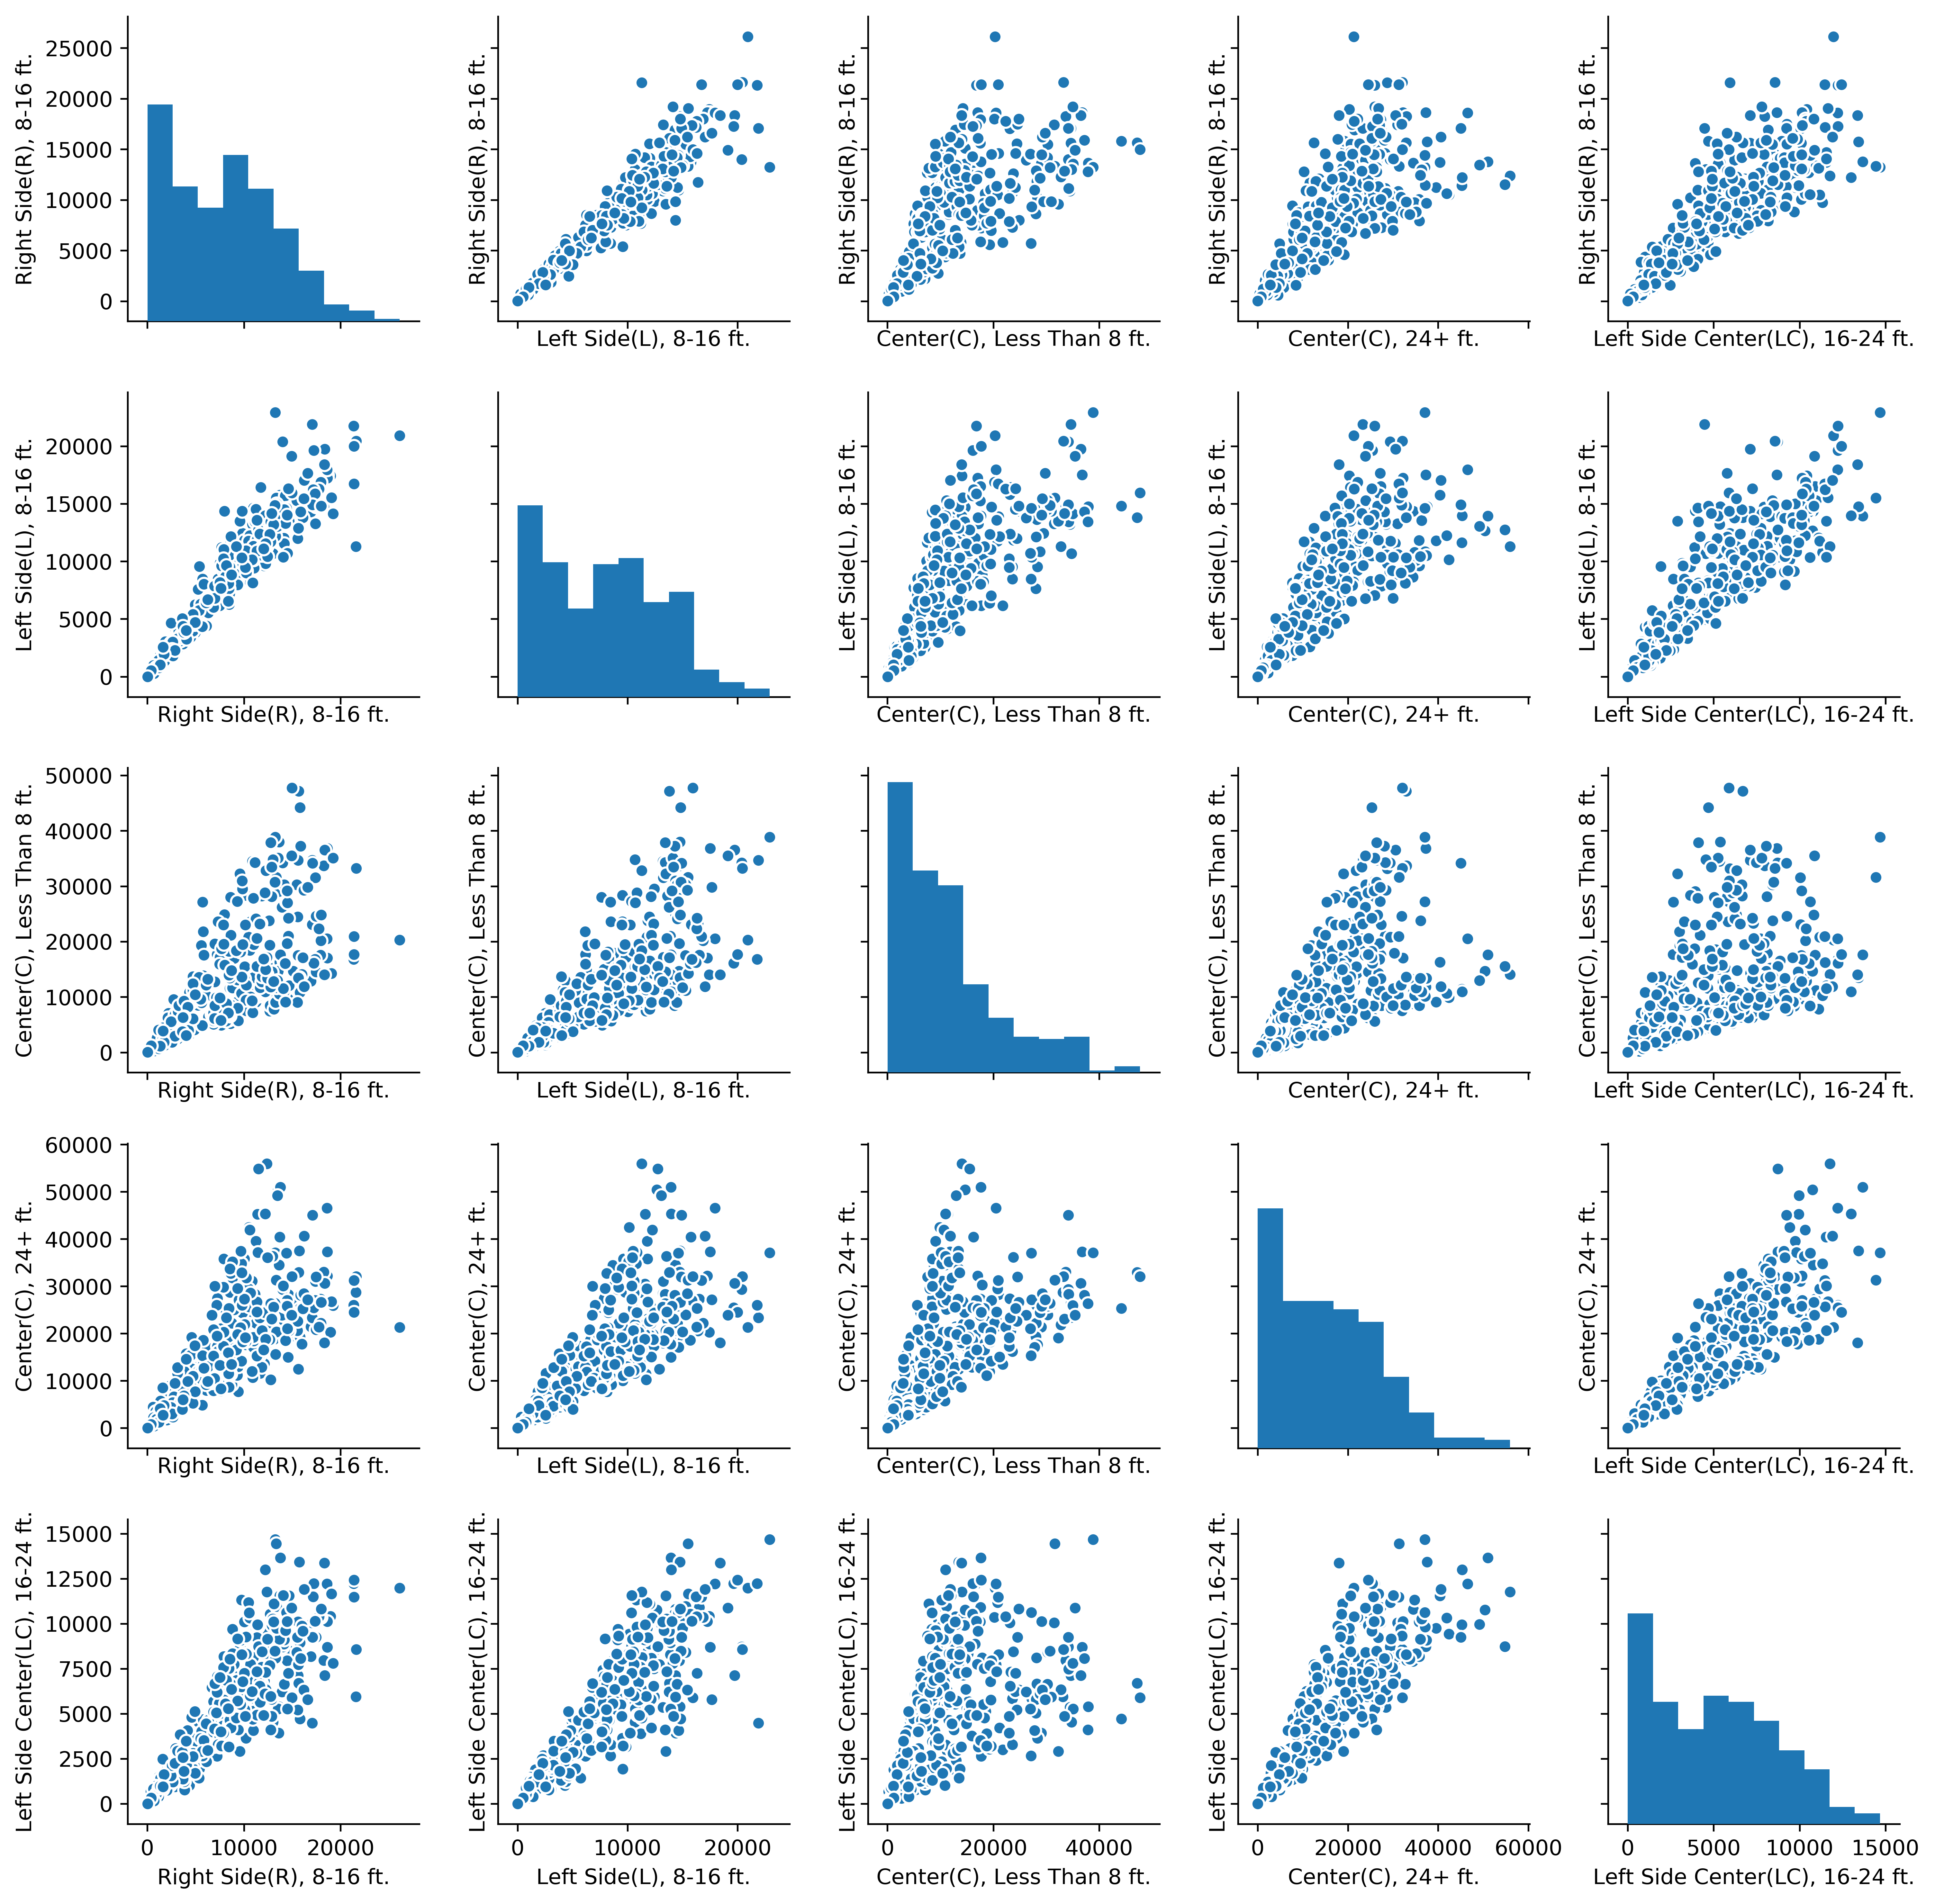
\includegraphics[width=0.80000\textwidth]{player_dist_and_relationships.png}
\caption{Relationships between court locations, and their distributions
for players on offense}
\end{figure}

\section{Multivariate Analysis and discussion of
results}\label{multivariate-analysis-and-discussion-of-results}

\subsection{Factor analysis and PCA: distinguishing players and teams
based on court
locations}\label{factor-analysis-and-pca-distinguishing-players-and-teams-based-on-court-locations}

First, we will use factor analysis to try and identify court locations
that differentiate teams and players from one another. The results that
made the most sense came from running factor analysis on a matrix that
had been normalized across rows, so that each value corresponding to one
of the position parameters represented the probability of a player/team
being in that position, instead of being a raw count. We used Sci-Kit
Learn's Factor Analysis implementation, since we could only create the
plots used below in python (we had to develop a custom plot ourselves
using python's matplotlib package).

\subsubsection{Players}\label{players}

First, we ran a PCA to decide how many loadings to use (for the matrices
of counts for offense and defense separately). A simple elbow plot
suggested that most of of the variance could be explained by the first
two loadings for both offense and defense. Because there are many unique
play-styles in the NBA, we decided to go ahead and use four components
-- explaining the style of a couple players with really unique styles in
our model isn't a bad thing.

\begin{figure}
\centering
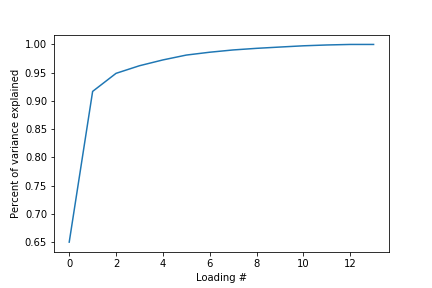
\includegraphics{cum_pca_offense.png}
\caption{Cumulative explained variance, PCA, on offense data}
\end{figure}

Then, we used Factor Analysis on a correlation matrix of the data. We
chose a correlation matrix because there is such a playtime difference
between players, and we didn't want this to bias our data. We don't have
to worry about accidentally biasing our data because we have plenty of
data on a player even if they spend only minutes on the court.

The results are plotted below. Each element in the loading vector
corresponds to a court location, so we have plotted this value on an
actual court. Larger values (red in the plot) in a loading vector mean
that players that have a higher score for this factor will tend to be in
the corresponding area a lot, and smaller values (blue) indicate that a
player has a tendency to not be in those regions. We think of these
loading values as characterizing the play style of players: For example,
a larger value in the loading vector element corresponding with ``Right
Side(R), 8-16 ft.'' means that this the play style corresponding with
this loading characterized by playing a lot in this zone.

\paragraph{Offense}\label{offense}

First, we look at what locations distinguish players from each other on
offense. The factor analysis seems to suggest that there are two play
styles that characterize basketball players in the NBA:

\begin{figure}
\centering
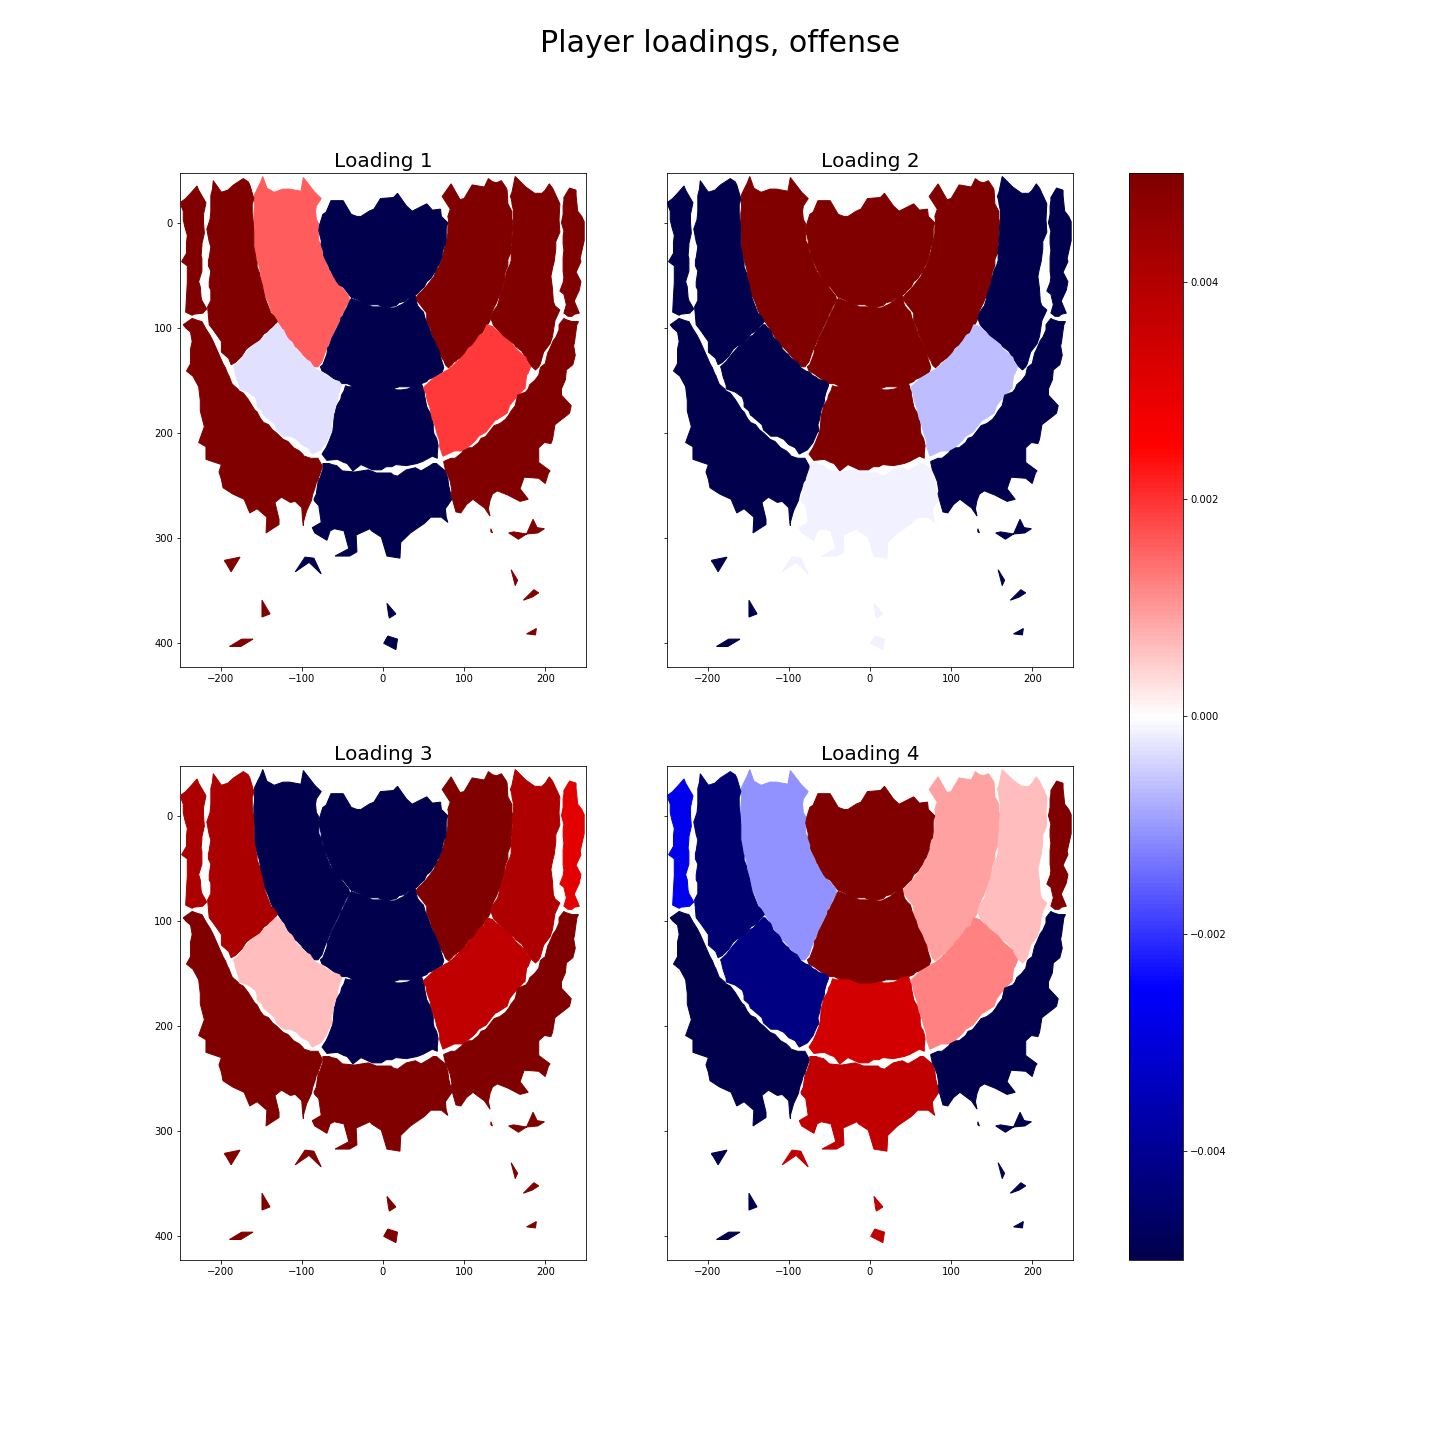
\includegraphics[width=0.80000\textwidth]{first_4_loadings_players_off.png}
\caption{Plot of loadings for players on offense}
\end{figure}

\begin{itemize}
\item
  The first loading, is a player who stays in areas around the
  perimeter. These are likely players like guards and small forwards.
\item
  The second loading likely represents players like centers, who
  penetrate the center of the court and attack the rim: It is
  characterized by large values for zones close to the basket.
\item
  The third loading seems similar to the first, with the addition of the
  center. It is probably detecting guards and avoiding the noise
  surrounding many people running through the middle of the court
\item
  The fourth loading seems similar to the second, with the addition of
  perimeter shooting. It could be telling us that there are players who
  play in the middle and shoot from the perimeter, even though many of
  these players, like Joel Embiid, do exist.
\end{itemize}

It is very interesting to see that perimeter players are not
characterized by being in the center back-court. This is likely because
so players of all types pass through the center to get from one side of
the court to another, not because perimeter players never spend time in
the center of the back-court.

\paragraph{Defense}\label{defense}

Next, we look at what locations distinguish players from each other on
defense. A plot of cumulative variance explained for the PCA again
suggests that there will be up to 6 significant loadings.

The loadings for the factor analysis on defense are much less repetitive
than those on offense. All of the first four loadings have some unique
characteristics.

\begin{figure}
\centering
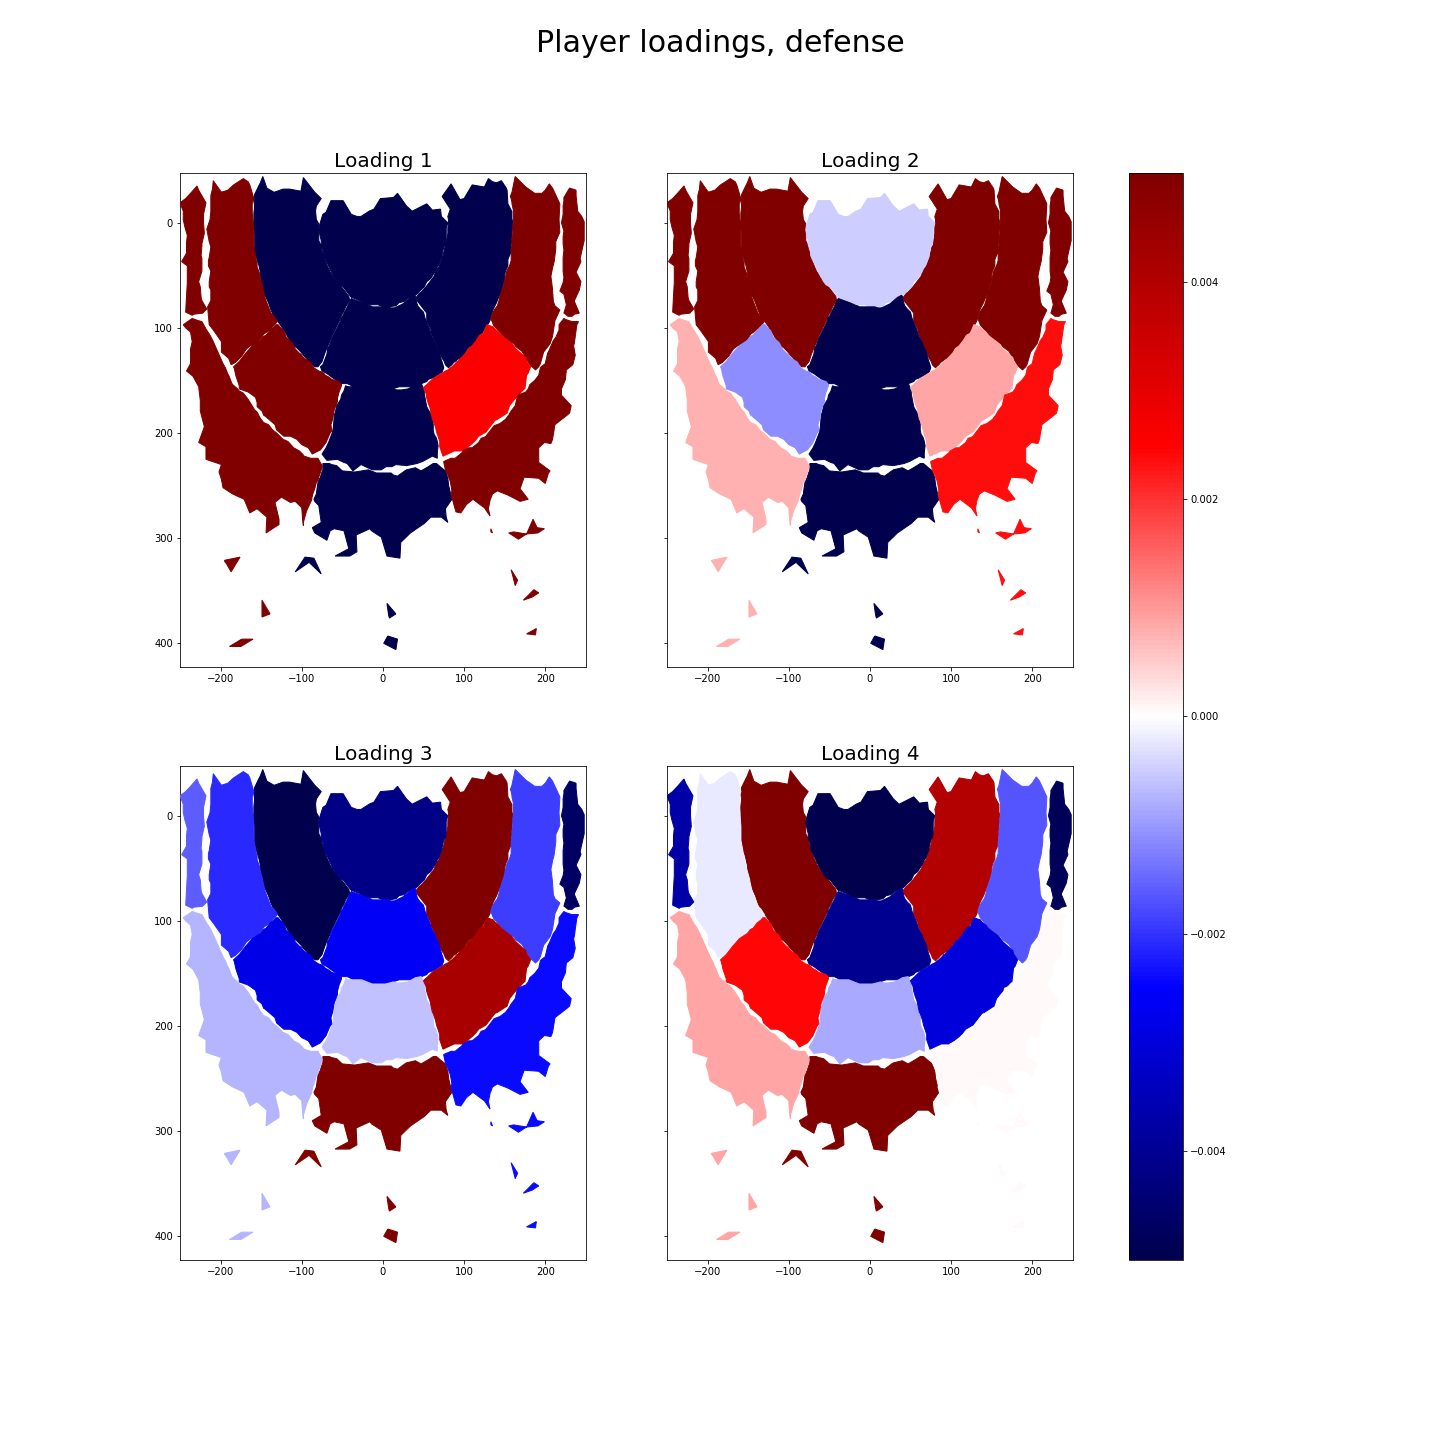
\includegraphics[width=0.80000\textwidth]{first_4_loadings_players_def.png}
\caption{Plot of loadings for players on defense}
\end{figure}

\begin{itemize}
\item
  The first loading appears to correspond with players who defend the
  sides of the court. It suggests that such players are generally
  ambidextrous in their ability to defend sides of the court. It is
  interesting to note how such players will often defend all the way up
  to the net against players on the far right or left. This is likely
  because players are less concentrated in these areas, and thus one man
  needs to cover more area on the right or left.
\item
  The second loading likely corresponds with players like center who
  defend the rim and spend a lot of time underneath the basket.
\item
  The third loading, if it is to be trusted, seems to correspond with a
  free-ranging type of player on defense, with scatterings of hot spots
  all over the court.
\item
  The fourth loading seems to be a player heavily focused on defending
  the perimeter, especially the far right and left regions of the court.
  It is believable that only certain types of players are likely to
  defend these regions--a taller player would not want to be drawn so
  far away from the basket, so it likely falls upon the smaller players
  to defend these far-drawn regions of the court.
\end{itemize}

\subsubsection{Teams}\label{teams}

\paragraph{Offense}\label{offense-1}

\begin{figure}
\centering
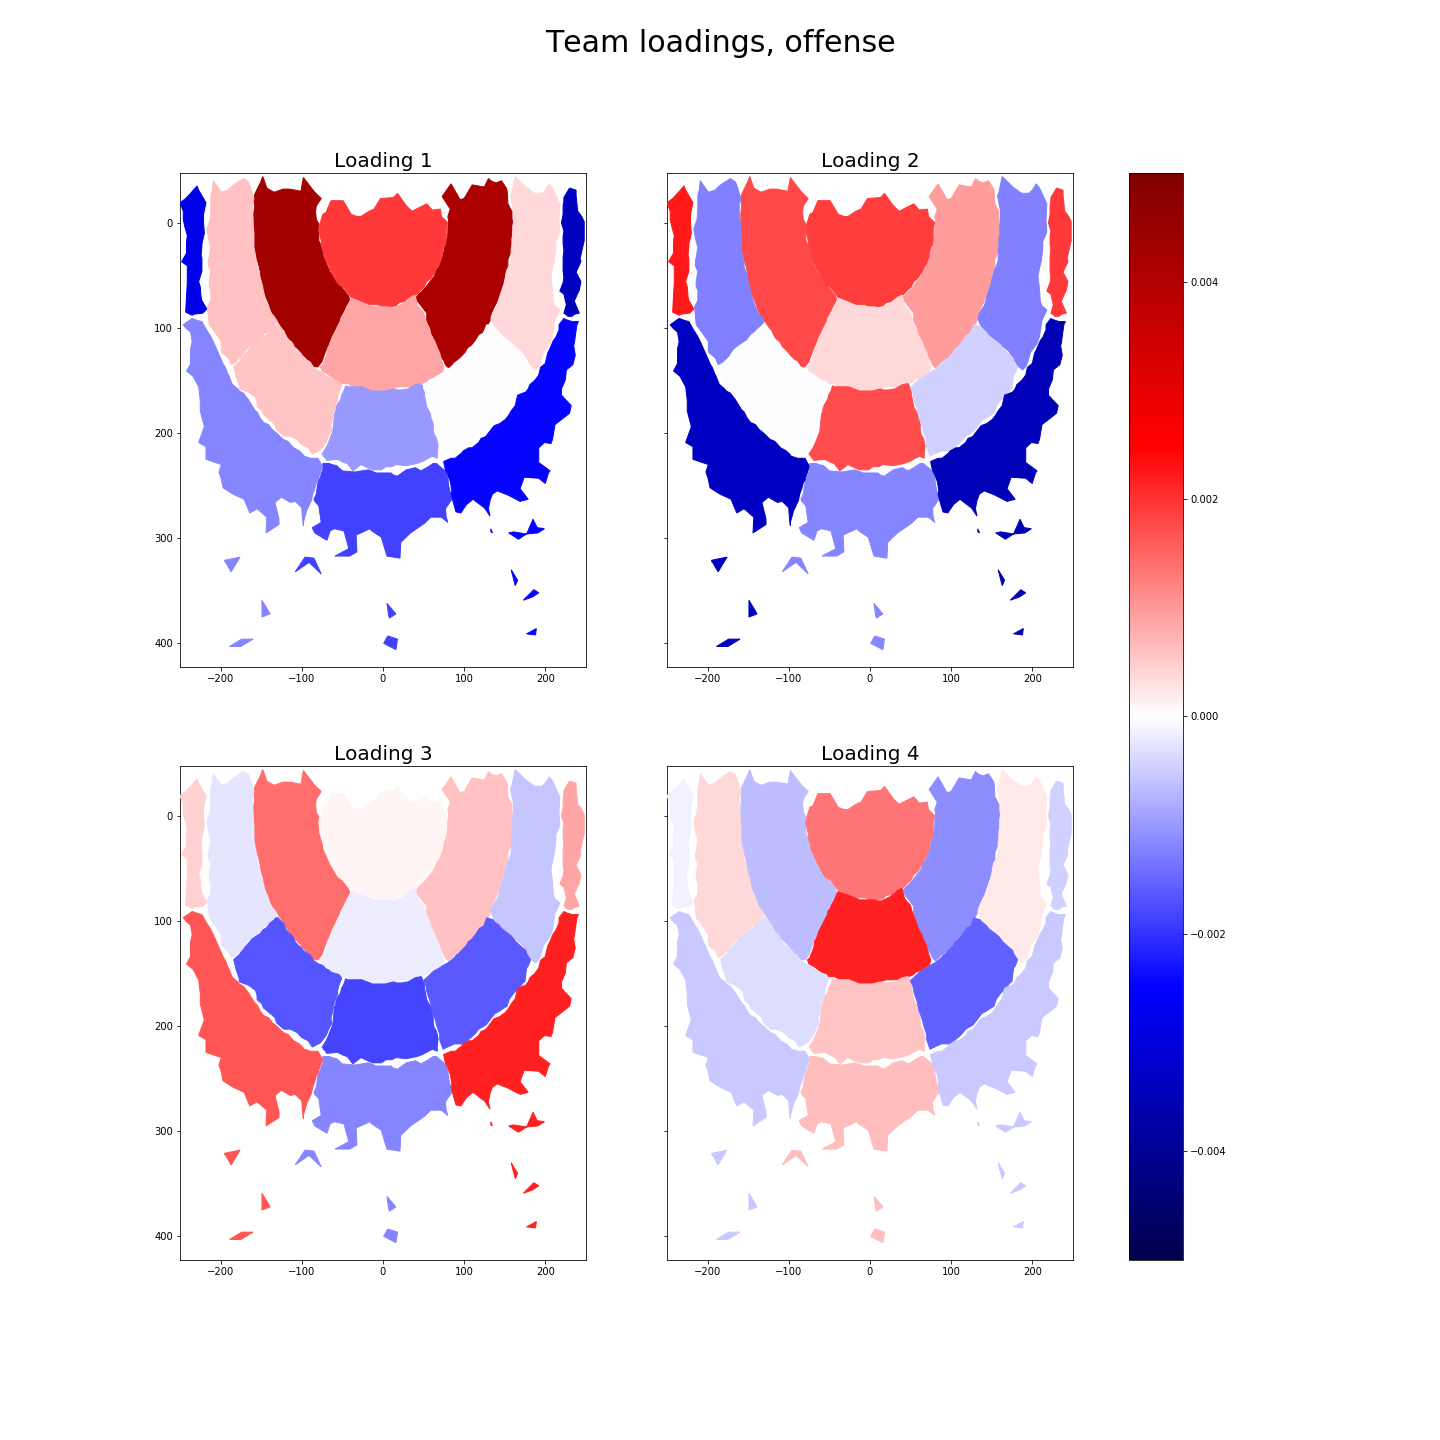
\includegraphics[width=0.80000\textwidth]{first_4_loadings_teams_off.png}
\caption{Plot of loadings for teams on offense}
\end{figure}

We perform the same analysis as above, just on a matrix with teams,
rather than players, as data points. This analysis is likely less
stable, since there are only 30 or so teams in the NBA, and we use
fourteen court locations, so the number of features is closer to the
number of data than ideal. In contrast with the PCA performed on the
players, the cumulative explained variance plot for teams does not reach
90\% until the fourth loading.

For offense, we see that some teams are more characterized by their
internal play, which makes up the first loading, while others are more
by their perimeter play, indicated by the the third loading. The team
play styles characterized the the second and fourth loading plots seem
to be offenses that are fairly evenly balanced across zones.

It is interesting to see how much more important interior play is on the
team level -- the first two loadings are heavily comprised of it. It
also makes sense to see perimeter play highlighted in the third, rather
than the first or second loadings, since only a few teams in the NBA,
like the Houston Rockets and Golden State Warriors, are heavily reliant
on their perimeter game, and so a relatively smaller amount of the
variance in the data is explained by playing in these zones.

\paragraph{Defense}\label{defense-1}

\begin{figure}
\centering
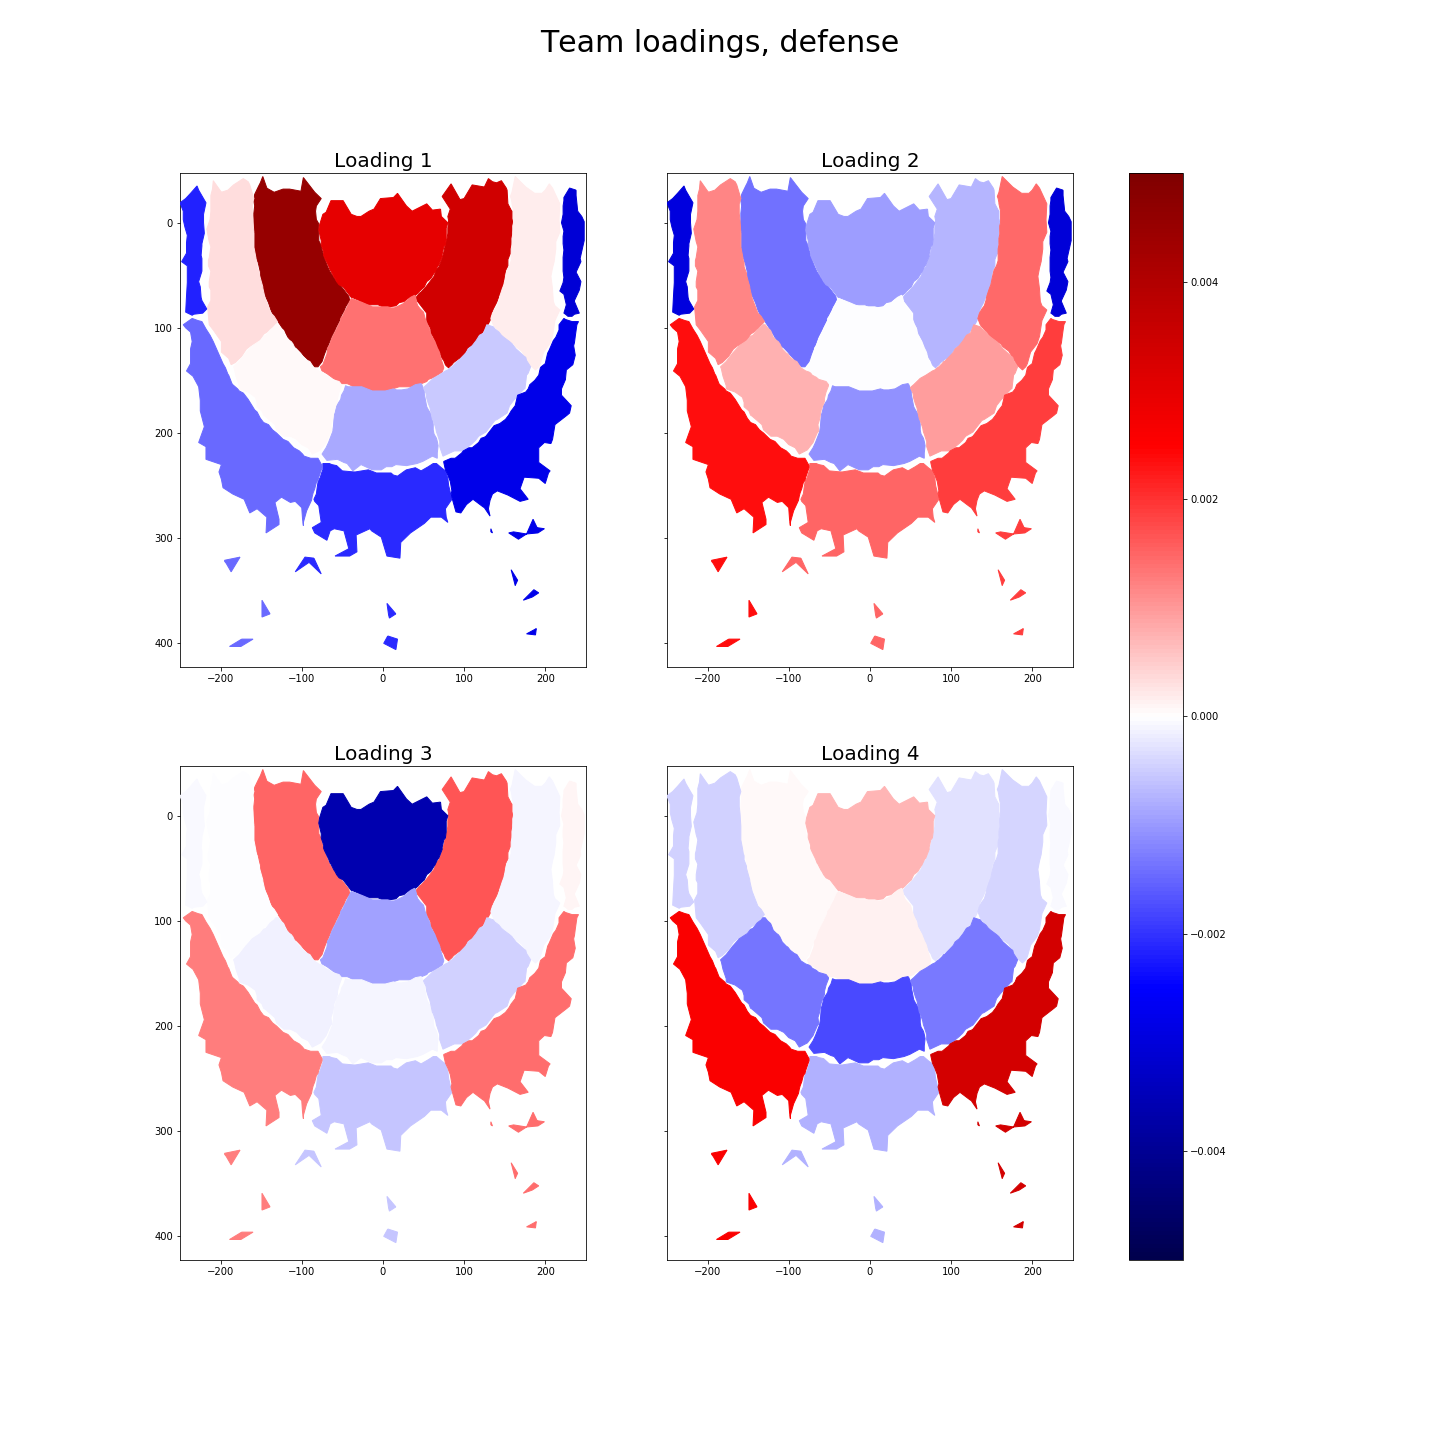
\includegraphics[width=0.80000\textwidth]{first_4_loadings_teams_def.png}
\caption{Plot of loadings for teams on defense}
\end{figure}

The defensive loadings show that some teams rely heavily on their
interior defense close to the net, while others (the second loading)
have a much more spread out defensive scheme. Loading three is
especially interesting, indicating that some teams almost never play
defense directly under the net. This could be teams like the Warriors,
who don't have an established big man to protect their rim, but do have
plenty of players in the 6'6 - 6'9 range who can play around the rim. It
also might just indicate that some teams don't like to risk jumping in
the way of some driving to the rim for a dunk, which risks a high-speed
midair collision.

\subsection{MANOVA: Examining the effect team has on court location for
players.}\label{manova-examining-the-effect-team-has-on-court-location-for-players.}

People often say that NBA teams like the Spurs have distinctive play
styles--``systems''. This section will try and verify this claim using
Multivariate Analysis of Variance to search for a relationship between
team and the locations players stand in on the court.

We find\ldots{}

To examine how much of a role the team plays in determining what zones
people spend time in.

\section{Conclusions and Discussion}\label{conclusions-and-discussion}

In conclusion, we find that movement data can characterize player
styles.

\section{Points for further analysis}\label{points-for-further-analysis}

Although looking at where players were at a single point in time told us
a lot about NBA games, looking at their transitions could potentially
tell us even more. This type of data, which would be very high
dimensional, would not be a good candidate for factor analysis or PCA,
since the number of features would outstrip the number of players or
teams. It would, however work very well for clustering analyses. If we
had time and space for another analysis, we would like to delve into

It would also be interesting for someone with more in depth knowledge of
players in the NBA to go through and inspect what factors specific
players scored high in. Would a player like Stephen Curry, the NBA MVP
who is known for his three point shooting, have high factor scores with
respect to zones outside of the three point arc?

\section{Data}\label{data-1}

Data is available in the \texttt{data} folder of the following github
repository: \url{https://github.com/samghelms/nba_movement_analysis}.
The following notebook walks through the analyses we used to create the
plots in this report.

\end{document}
